\documentclass[review,10pt]{elsarticle}
\usepackage[utf8]{inputenc}
\usepackage{microtype}
\usepackage[margin=2.5cm]{geometry}
\usepackage{setspace}
\setstretch{1.5}
\usepackage[none]{hyphenat}
\usepackage[pagewise]{lineno}
\usepackage[english]{babel}
\usepackage[table]{xcolor}
\usepackage{soul}
\usepackage{tikz}
\usepackage{booktabs}
\usepackage{longtable}
\usepackage{array}
\usepackage{etoolbox}
\usepackage[most]{tcolorbox}
\usepackage{ragged2e}
\usepackage[overload]{empheq}
\usepackage[justification=justified]{caption}
\usepackage{enumitem}
\newtheorem{proposition}{Proposition}
\newtheorem{property}{Property}
\newtheorem{corollary}{Corollary}
\newtheorem{lemma}{Lemma}
\newtheorem{definition}{Definition}
\newtheorem{theorem}{Theorem}
\usepackage{amsmath,amsfonts,amssymb,mathtools}
\usepackage{cases}
\usepackage{multirow}
\usepackage{graphicx,float}
\usepackage{algpseudocode}
\usepackage{subcaption}
\usepackage{eurosym}
\usepackage{amstext}
\usepackage{arydshln}
\usepackage{flushend}
\usepackage{threeparttable}
\usepackage{url}
\usepackage{mdframed}
\usepackage[]{hyperref}
\hypersetup{colorlinks, linkcolor=blue, citecolor=blue, urlcolor=blue}
\usepackage{xurl}

\setlength{\LTcapwidth}{0.92\textwidth}
\newcolumntype{L}[1]{>{\RaggedRight\arraybackslash}p{#1}}
\AtBeginEnvironment{longtable}{%
  \footnotesize
  \setlength{\tabcolsep}{2.8pt}
  \renewcommand{\arraystretch}{1.12}
}
\captionsetup[longtable]{font=footnotesize,labelfont=bf,singlelinecheck=false}

\DeclareMathOperator*{\argmax}{arg\,max}
\DeclareMathOperator*{\argmin}{arg\,min}

\usepackage[ruled,vlined,linesnumbered]{algorithm2e}
\DeclareRobustCommand{\officialeuro}{%
  \ifmmode\expandafter\text\fi
  {\fontencoding{U}\fontfamily{eurosym}\selectfont e}}
\usepackage{framed}

\usepackage{multicol}
\usepackage{nomencl}[noprefix]
\makenomenclature
\setlength{\nomitemsep}{-\parskip}

\renewcommand*\nompreamble{\begin{multicols}{2}}
\renewcommand*\nompostamble{\end{multicols}}

% Revision macros retained for compatibility; this clean version applies no highlighting.
\newcommand{\revpar}[1]{#1\par\medskip}
\newcommand{\revtitle}[1]{#1}
\DeclareRobustCommand{\change}[1]{#1}
\newcommand{\changepar}[1]{#1\par\medskip}

\begin{document}

\justifying
\begin{frontmatter}

\title{\revtitle{Assessing Plastic-Packaging Circularity in Chile: EPR Performance, Data Gaps, and Measurement Readiness}}

\author[1]{Catalina Arriagada}
\author[1]{Ivan Derpich\corref{cor1}}
\ead{ivan.derpich@usach.cl}
\cortext[cor1]{Corresponding author.}
\author[1]{Andrés Viveros}
\author[1]{Juan Miguel Sepúlveda}
\address{Departamento de Ingeniería Industrial, Universidad de Santiago de Chile, Santiago, Chile}

\begin{abstract}
\revpar{Extended Producer Responsibility (EPR) systems require reliable information not only on collected and recovered waste, but also on whether recovered materials effectively return to production. This study examines what publicly accessible information can reveal about Chile's plastic-packaging system and whether the national information infrastructure supports a methodologically defensible circularity assessment. National series for 2015--2025 were used to estimate total and packaging recycling rates, EPR target attainment, the ratio of managed material to virgin-resin input, and the theoretical potential for greenhouse-gas impact reduction. A structured public-source audit assessed seven measurement applications against ten dimensions of data readiness and classified them as Available, Partial, or Insufficient without aggregating them into a composite score. For the 2024 reference year, total-plastics and plastic-packaging recycling rates were estimated at 10.3\% and 13.0\%, respectively, while estimated EPR target attainment reached 82.0\%. For PET, PP, and PE, managed material represented 21.9\%, 31.9\%, and 16.9\% of virgin-resin input, respectively. Under one-to-one substitution assumptions and transferred emission factors, the aggregate theoretical Impact Reduction Potential was 0.175 Mt CO$_2$eq. The audit classified aggregate total-plastics recycling as Available; packaging recycling, estimated EPR attainment, eC, and IRP as Partial; and a complete MCI and minimum national material-flow account as Insufficient. The limiting variables were compatible recycled inputs, unrecovered waste, process losses, final material destinations, and product utility. Chile's public information infrastructure therefore permits selected mass-based estimates but not a comprehensive national circularity account.}
\end{abstract}

\begin{keyword}
circularity measurement; plastic packaging; extended producer responsibility; data availability; Material Circularity Indicator; Chile; material-flow traceability
\end{keyword}

\end{frontmatter}

\section{Introduction}

\revpar{Global plastic production increased from 2 million tonnes in 1950 to approximately 370-380 million tonnes in 2020 (Van der Perre et al., 2024), driven by the durability, versatility, and low cost of plastic materials. Yet only 9\% of plastics produced historically have been recycled, while 79\% have been discarded in landfills or released into the environment (Schwarz et al., 2021). Beyond waste management, plastics are also relevant to the climate crisis: in 2019, the plastics system generated nearly 1.8 billion tonnes of greenhouse gas emissions, equivalent to 3.4\% of global emissions, and this figure could triple by 2050 if production and consumption patterns remain unchanged (Van der Perre et al., 2024).}

\revpar{The circular economy seeks to decouple economic growth from the consumption of natural resources (\change{Corona et al., 2019}), replacing the linear take-make-dispose model with strategies based on reduction, reuse, recycling, and material recovery (Olatayo et al., 2023). Measuring this transition using reliable data is critical for public policy design (\change{Corona et al., 2019}), particularly because the literature emphasizes that higher circularity does not automatically imply higher environmental sustainability (Rigamonti and Mancini, 2021; Vadoudi et al., 2022). Recycling rates alone therefore cannot determine whether a system effectively reduces its material and environmental impacts.}

\revpar{Circular-economy measurement is itself a data-governance problem. Indicator reviews show that circularity metrics differ in scale, system boundary, circular strategy, and whether they describe actual or potential performance (Saidani et al., 2019; Kristensen and Mosgaard, 2020). At national scale, the OECD distinguishes operational indicators that can be produced with established data from aspirational indicators that require further statistical and methodological development (OECD, 2024). It also emphasizes that material-flow accounts must connect waste, product, trade, and environmental-economic information. Consequently, the existence of isolated datasets does not establish measurement readiness: the variables must be accessible, sufficiently granular, temporally continuous, and interoperable at a common boundary.}

\changepar{Extended Producer Responsibility (EPR) is one of the most widely adopted environmental policy instruments for financing and organizing packaging-waste recovery, shifting costs that would otherwise fall on municipalities or the state toward producers (Andreasi Bassi et al., 2020). EPR systems differ substantially across countries in target ambition, coverage scope, traceability mechanisms, and enforcement incentives. In the European Union, Directive (EU) 2018/852 requires 50\% recycling of plastic packaging by 2025 and 55\% by 2030 (Picuno et al., 2021; Van der Perre et al., 2024). Germany exceeds 40\% effective recycling through dense separate-collection systems and deposit-refund schemes, while the Netherlands reaches approximately 30\% despite advanced infrastructure (Picuno et al., 2021). Portugal is a relevant comparator for the Chilean context because recent studies have applied MFA and circularity indicators to national plastic systems (Goncalves et al., 2024; Goncalves et al., 2026).}

\revpar{In Chile, Law No. 20.920 (the EPR Law) defines priority products according to mass consumption, hazard, or recovery potential, including packaging. Supreme Decree No. 12/2020 establishes collection and recovery targets that producers generally meet through collective management systems. The Chilean EPR framework shares the principle of assigning responsibility to producers, but it remains at an earlier stage of implementation, with more conservative targets and less publicly disaggregated data than those available in Europe. While the Chilean operational focus is still centered on accrediting tonnes collected and recovered, international research, including material flow analysis (MFA) studies for Spain (Lopez-Aguilar et al., 2022) and Portugal (Goncalves et al., 2024), has moved toward indicators of recycled content, material circularity, and environmental impact. More mature systems are therefore distinguished not only by recycling more material, but also by measuring more accurately what happens to materials after collection (Antonopoulos et al., 2021).}

\revpar{This study focuses on plastic packaging, a key fraction of the packaging system due to its use in food, beverages, cleaning products, hygiene products, and e-commerce. Its recovery potential depends on resin type, color, contamination, and product design (Antonopoulos et al., 2021; \change{Eriksen and Astrup, 2019}). In Chile, \change{ASIPLA (2025b) reports that 88\% of recycled plastic comes from industrial and commercial sources, while only 12\% originates from household sources}. National reports tend to describe collection volumes, but quantitative evidence on how these flows affect material circularity and the country's environmental footprint remains limited (Goncalves et al., 2024; Lopez-Aguilar et al., 2022).}

\changepar{This study addresses two co-primary research questions. First, to what extent do the publicly accessible governmental and sectoral data examined enable a transparent and methodologically defensible assessment of plastic-packaging circularity in Chile (RQ1)? Second, what do the indicators that can currently be calculated reveal about the evolution and divergence of recovery performance, estimated EPR target attainment, managed material relative to virgin-resin input, and theoretical impact-reduction potential during 2015--2025 (RQ2)? To answer these questions, the analytical framework combines total and packaging recycling rates (TR), an estimated packaging-generation scale ($T_{gr}$), an estimated EPR target-attainment indicator (IC$_{\mathrm{REP,est}}$), a resin-level managed-to-virgin material ratio reported as eC, and Impact Reduction Potential (IRP). The MCI is used as a demanding data-feasibility test rather than calculated through unsupported assumptions. The study consequently distinguishes what can be observed, what can only be estimated, and what cannot yet be calculated at a consistent national boundary.}

\revpar{To establish the institutional setting in which these indicators operate, Table \ref{tab:actores_rep_chile} identifies the principal stakeholders in the Chilean EPR value chain. The first column names and numbers each stakeholder, while the second specifies its operational, financial, regulatory, or monitoring role. The numbering is retained in Figure \ref{fig:actores}, allowing the institutional descriptions in the table to be matched directly with the relationships shown in the diagram.}

\begin{longtable}{|L{4.5cm}|L{10cm}|}
\caption{Actors in the EPR value chain in Chile}
\label{tab:actores_rep_chile}\\
\hline
\textbf{Stakeholder} & \textbf{Role in the value chain} \\
\hline
\endfirsthead
\hline
\tikz[baseline=(char.base)]{\node[draw,circle,inner sep=1pt] (char) {\textbf{1}};} Producers and importers & Place packaged products on the domestic market. They must declare the packaging they introduce, finance its management, and comply with EPR targets. \\
\hline
\tikz[baseline=(char.base)]{\node[draw,circle,inner sep=1pt] (char) {\textbf{2}};} Management systems & Nonprofit organizations or authorized individual systems that group producers and implement collection and recovery plans. \\
\hline
\tikz[baseline=(char.base)]{\node[draw,circle,inner sep=1pt] (char) {\textbf{3}};} Waste pickers & Collect, separate, sort, and sell recyclable waste for subsequent recovery. They may work independently or be integrated into management systems.\\
\hline
\tikz[baseline=(char.base)]{\node[draw,circle,inner sep=1pt] (char) {\textbf{4}};} Collection operators & Collect waste from households, recycling centers, businesses, and industrial facilities. \\
\hline
\tikz[baseline=(char.base)]{\node[draw,circle,inner sep=1pt] (char) {\textbf{5}};} Transportation operators & Transport waste from the point of generation to sorting or recovery facilities. \\
\hline
\tikz[baseline=(char.base)]{\node[draw,circle,inner sep=1pt] (char) {\textbf{6}};} Storage operators & Receive and temporarily store waste before treatment or transfer to another facility. \\
\hline
\tikz[baseline=(char.base)]{\node[draw,circle,inner sep=1pt] (char) {\textbf{7}};} Pre-treatment or sorting operators & Separate materials by type, remove impurities, and compact or bale waste to prepare it for recycling. \\
\hline
\tikz[baseline=(char.base)]{\node[draw,circle,inner sep=1pt] (char) {\textbf{8}};} Recovery operators & Recover value from waste through recycling or other recovery processes.\\
\hline
\tikz[baseline=(char.base)]{\node[draw,circle,inner sep=1pt] (char) {\textbf{9}};} Disposal operators & Carry out final disposal of waste that cannot be recovered. \\
\hline
\tikz[baseline=(char.base)]{\node[draw,circle,inner sep=1pt] (char) {\textbf{10}};} Municipalities & Coordinate local household-waste collection, recycling centers, and public-education initiatives in collaboration with management systems. \\
\hline
\tikz[baseline=(char.base)]{\node[draw,circle,inner sep=1pt] (char) {\textbf{11}};} Consumers & Separate waste and deliver packaging to designated collection points. Their behavior directly affects the quality of recovered material. \\
\hline
\tikz[baseline=(char.base)]{\node[draw,circle,inner sep=1pt] (char) {\textbf{12}};} Ministry of the Environment (MMA) & Issues decrees establishing targets, reviews and authorizes management plans, and coordinates regulatory implementation.\\
\hline
\tikz[baseline=(char.base)]{\node[draw,circle,inner sep=1pt] (char) {\textbf{13}};} Superintendency of the Environment & Monitors compliance with obligations, traceability requirements, reporting duties, and established targets, and may initiate enforcement proceedings. \\
\hline

\end{longtable}

\revpar{Table \ref{tab:actores_rep_chile} shows that packaging recovery is not performed by a single actor. Producers and importers finance compliance; management systems coordinate implementation; consumers, waste pickers, and collection and treatment operators move materials through the chain; municipalities provide territorial coordination; and environmental authorities regulate and supervise the system. This division of responsibilities is relevant to the indicator framework because reported recovery depends on both physical material flows and the institutional mechanisms used to finance, document, and verify them.}

\revpar{Figure \ref{fig:actores} translates the stakeholder list into a process map. It should be read from producers and consumers toward collection, transport, storage, pre-treatment, recovery, and final disposal. The arrows distinguish the physical flow of waste from financing, regulatory, oversight, territorial-coordination, participation, and reporting relationships, as detailed in the figure legend.}

\begin{figure}[H]
    \centering
    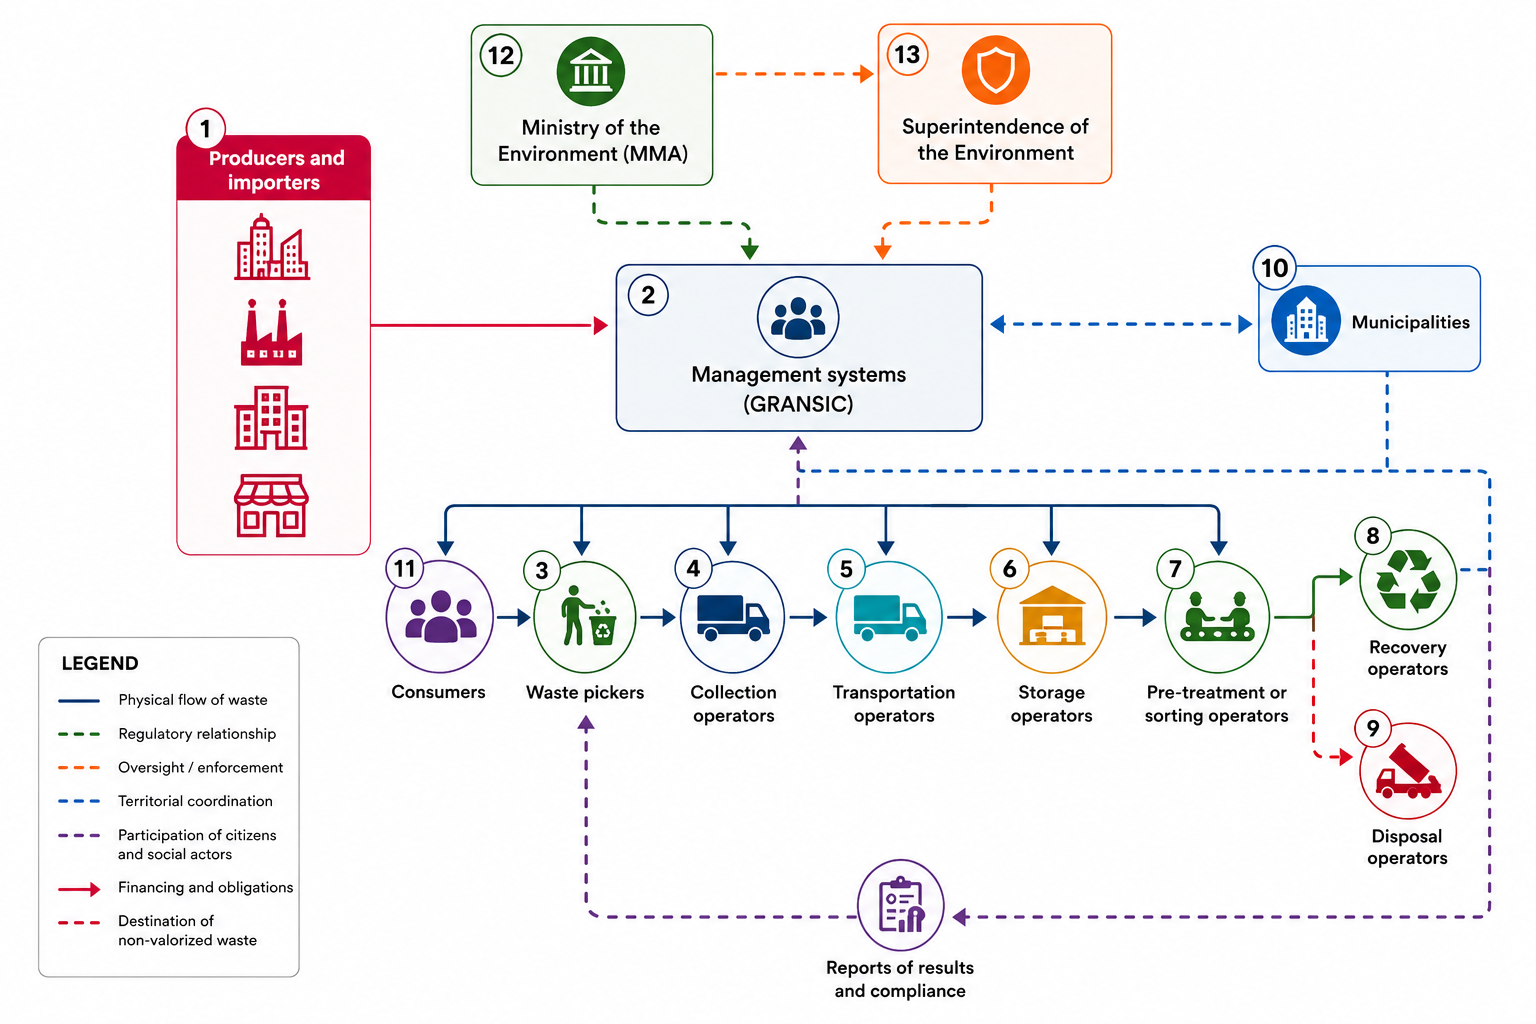
\includegraphics[width=1.0\textwidth]{../figuras/actores_rep_chile.png}
    \caption{Institutional actors and material, financial, regulatory, and reporting relationships in the Chilean EPR value chain.}
    \label{fig:actores}
\end{figure}

\revpar{The process map clarifies why a mass-based recovery result alone cannot describe system circularity: material may be collected and formally reported without demonstrating its quality, reinsertion into production, or substitution of virgin resin. This institutional distinction motivates the combined use of operational, material-circularity, and environmental indicators in the remainder of the study.}

\revpar{For comparative context, Table \ref{tab:modelos_internacionales} summarizes selected EPR and circular-economy applications discussed in the literature. The first column identifies the country or region, the second describes the dominant policy or analytical approach, and the third records the element most relevant to the Chilean case, such as traceability, sorting quality, material-flow analysis, or environmental assessment.}

\begin{longtable}{|L{3cm}|L{6cm}|L{6cm}|}
\caption{International models}
\label{tab:modelos_internacionales}\\

\hline
\textbf{Country/region} & \textbf{EPR or circular approach} & \textbf{Key elements identified in the literature} \\
\hline
\endfirsthead

\hline
European Union & Recovery and recycling targets with strong institutional traceability. & Post-consumer flows depend on effective recovery, sorting quality, and secondary markets (Antonopoulos et al., 2021).\\
\hline
Austria & Mature packaging system with circular-practice assessment. & Packaging circularity depends on composition, collection, sorting, and recycling routes (Picuno et al., 2021). \\
\hline
Germany and the Netherlands & EPR systems with high coordination and comparative performance. & Institutional and operational factors explain differences between packaging systems (Picuno et al., 2021). \\
\hline
Spain & Use of MFA to assess end-of-life packaging management. & Data gaps make it difficult to measure effective recyclability and real circularity (Lopez-Aguilar et al., 2022).\\
\hline
Portugal & MFA and circularity assessment applied to plastic packaging. & Circularity depends on material flows, reinsertion, and substitution of virgin material (Goncalves et al., 2024; Goncalves et al., 2026). \\
\hline
Norway & Environmental assessment of ambitious targets and increased separation/sorting. & Increasing separation may provide benefits, but must be assessed against environmental impacts (Klotz et al., 2023). \\
\hline
Colombia & Environmental validation of packaging recovery systems through LCA. & \change{Restrepo et al. (2026) assess the Circular Vision packaging recovery system using LCA and primary operational data for multiple packaging material streams.}\\
\hline

\end{longtable}

\revpar{The comparison in Table \ref{tab:modelos_internacionales} indicates that higher collection or recycling targets are most informative when accompanied by reliable traceability, sorting-quality information, secondary-material markets, and environmental evaluation. The table is not intended as a league table of national performance; rather, it identifies design features and analytical practices that inform the selection of indicators for Chile.}

\section{Literature Review and Research Gaps}

\revpar{The measurement of the circular economy has led to a proliferation of indicators. \change{Corona et al. (2019)} identify multiple indices, indicators, and frameworks, none of which fully capture multiple material cycles or the consequences of downcycling. The Material Circularity Indicator (MCI), developed by the Ellen MacArthur Foundation (2015), is among the most widely adopted product- and firm-level indicators. It measures the minimization of linear flows on a scale from 0 to 1 (Rigamonti and Mancini, 2021). Its main limitation for the present study is that it was originally designed for product-level assessment rather than national system-level analysis. Recent adaptations have extended its use, including Vadoudi et al. (2022) for multilayer packaging and Goncalves et al. (2026) for total plastic flows in Portugal using MFA.}

\changepar{Schulte et al. (2023) propose complementary circularity and environmental indicators for polypropylene in a European context. From that framework, the present study adopts eC and IRP while testing their applicability to Chilean national data. Olatayo et al. (2023), in turn, propose eight key performance indicators for the recycling value chain; those eight indicators belong to their framework and are not the set calculated in the present study. Rigamonti and Mancini (2021) show that no circularity indicator should be used alone to select environmentally preferable options, because material circularity and environmental performance answer different questions. This provides the rationale for interpreting eC together with IRP and for treating MCI data feasibility as a separate methodological result.}

\revpar{The central research gap is not merely the absence of another national circularity score, but the limited evidence on whether emerging EPR information systems provide mutually compatible public variables for moving from mass-based recovery reporting to material-circularity assessment. Existing indicator taxonomies clarify what metrics are intended to measure (Saidani et al., 2019; Kristensen and Mosgaard, 2020), while national frameworks identify the need for interoperable material-flow information (OECD, 2024). However, fewer studies test whether the publicly accessible records of a recently implemented EPR system actually permit the selected indicators to be computed at consistent boundaries. The present study addresses that gap through a Chilean case that combines a structured readiness audit with the calculation of indicators supported by the available evidence. It identifies the boundary between estimated regulatory-performance monitoring and defensible material-circularity measurement rather than proposing a new indicator.}

\revpar{Table \ref{tab:comparacion_papers} organizes the positioning argument into three hierarchical gaps. The first is the principal methodological gap concerning computability and data readiness; the second is the empirical gap concerning Chile's early EPR implementation; and the third is the transferability gap concerning the minimum information architecture required beyond Chile. This hierarchy keeps IRP and the remaining calculated indicators as complementary evidence rather than separate novelty claims.}

\begin{longtable}{|L{5cm}|L{5cm}|L{5cm}|}
\caption{Research gaps and contribution of this study}
\label{tab:comparacion_papers}\\

\hline
\textbf{Identified gap} & \textbf{State of the literature} & \textbf{Contribution} \\
\hline
\endfirsthead

\hline
Computability and measurement readiness & Indicator taxonomies distinguish scales and purposes, while macro frameworks call for compatible material-flow accounts; neither guarantees that the necessary public variables can be linked in a recently implemented EPR system. & Applies an explicit public-source audit to seven measurement applications and identifies which variables, boundaries, and linkages permit or prevent calculation. \\
\hline
Chilean evidence during early EPR implementation & Latin American national evidence remains limited, and legal target reporting does not by itself demonstrate material reinsertion or environmental improvement. & Reports 2015--2025 operational estimates, with 2024 as the reference year, while separating estimated target attainment, managed-to-virgin material ratios, and theoretical IRP from official compliance and observed impact. \\
\hline
Transferable minimum information architecture & Circularity monitoring requires combinations of waste, material, product, trade, and destination information, but minimum cross-system data requirements are rarely made explicit in applied EPR assessments. & Derives a minimum reporting architecture linking placed-on-market mass, resin-level inputs, collection and recovery, process losses, final destinations, quality, and chain of custody. \\
\hline

\end{longtable}

\revpar{Taken together, the three rows in Table \ref{tab:comparacion_papers} establish a primary methodological contribution, a supporting Chilean empirical contribution, and a transferability contribution. The study applies existing metrics while keeping estimated and provisional inputs visible and declining to report a numerical MCI when the required variables cannot be supported.}

\revpar{Table \ref{tab:mapa_literatura} provides the detailed evidence map supporting that positioning. For each reference, the table reports the publication year and geographical setting, the plastic stream or resin studied, the principal indicators or methods, and the specific role of the source in the present manuscript. The final column is particularly important because it distinguishes sources used to define indicators from those used only for comparison, contextualization, or emission-factor inputs.}

{
\footnotesize
\renewcommand{\arraystretch}{0.75}
\begin{longtable}{|L{2cm}|L{2cm}|L{2.45cm}|L{2.55cm}|L{5cm}|}

\caption{Literature map: references, indicators, and role in the study}
\label{tab:mapa_literatura}\\

\hline
\textbf{Reference} &
\textbf{Year / country} &
\textbf{Plastic type} &
\textbf{Key indicators} &
\textbf{Role in this study} \\
\hline
\endfirsthead

\hline
\textbf{Reference} &
\textbf{Year / country} &
\textbf{Plastic type} &
\textbf{Key indicators} &
\textbf{Role in this study} \\
\hline
\endhead

Schulte et al. & 2023 / Germany & Polypropylene (PP) & eC, IRP &
Main source for the eC and IRP indicators selected for the analytical framework. \\
\hline

Sassanelli et al. & 2019 / Italy / global & Several plastics & MCI, Longevity Index &
Theoretical framework for circularity metrics and the need to integrate MCI with LCA. \\
\hline

Rigamonti and Mancini & 2021 / Italy & PET, PE, PP, PA, bioplastics & LCA, GWP &
Methodological support for combining circularity and environmental impact. \\
\hline

Olatayo et al. & 2023 / South Africa & Multiple packaging polymers & 8 performance KPIs &
Conceptual framework for diagnosing the maturity of the Chilean EPR system. \\
\hline

Dormer et al. & 2013 / Ireland & Recycled PET & Carbon footprint, GHG emissions &
Source informing emission factors for the IRP calculation. \\
\hline

Eriksen and Astrup & 2019 / Denmark & Source-separated rigid plastic waste &
Product design, polymer separability, colour, recycling quality &
Supports the statement that resin type, colour, contamination, product design, and separability affect recycling potential. \\
\hline

Goncalves et al. & 2026 / Portugal & General plastics & MCI, TR, MFA &
Direct comparator for national plastic-system MFA and circularity assessment in Portugal. \\
\hline

Aranda-Uson et al. & 2019 / Spain & Business circular-economy implementation &
Financial resources and regional policy implications &
Supports the need to consider enabling conditions for circular-economy implementation beyond physical recovery rates. \\
\hline

Vadoudi et al. & 2022 / France / Belgium & Multilayer packaging (PET, PUR, LDPE) &
Adapted MCI, LCA &
Supports adaptation of MCI to plastic-packaging systems. \\
\hline

Leal Filho et al. & 2025 / Estonia / Germany / EU & Multiple plastic resins &
GHG emission factors &
Source for resin-level emission factors used in the IRP calculation. \\
\hline

Restrepo et al. & 2026 / Colombia & Packaging material streams &
LCA, EPR recovery system, avoided impacts &
Supports the Latin American comparator on LCA-based validation of a packaging recovery system. \\
\hline

Saidani et al. & 2019 / international & Multiple sectors and scales &
Taxonomy of 55 circularity-indicator sets &
Supports explicit differentiation by scale, scope, circular strategy, and actual versus potential performance. \\
\hline

Kristensen and Mosgaard & 2020 / international & Micro-level circular-economy applications &
Critical review of 30 indicator approaches &
Supports the claim that indicator selection and interpretation remain non-standardized and scope dependent. \\
\hline

OECD & 2024 / national and subnational & Economy-wide materials and waste &
Operational and aspirational indicators; compatible MFA &
Supports the readiness framing and the need to link waste, material, product, trade, and environmental-economic data. \\
\hline

Solis and Silveira & 2020 / global & Household plastic waste &
Chemical-recycling technologies and TRL assessment &
Contextual basis for technological limits and maturity differences in plastic-recycling pathways. \\
\hline

\end{longtable}
}

\revpar{The literature map shows that no single source supplies the complete framework used here. Studies on MCI and MFA support material-flow measurement, EPR studies inform the institutional and regulatory dimension, and LCA or carbon-footprint studies support the environmental dimension. Their combination justifies a multidimensional assessment, but it also requires the boundaries of each adapted indicator to remain visible in the methodology.}

\section{Methodology}
\subsection{Research Design}

\changepar{This study uses a descriptive, quantitative system-level design to examine plastic-packaging recycling in Chile under Law No. 20.920 and a requirements-based assessment of whether the sources reviewed support circularity measurement. The compiled series covers 2015--2025. The year 2024 is designated as the reference year because it is the most recent year with the strongest joint coverage of apparent consumption, recycling, population, virgin material by resin, and managed material by resin. The 2025 results are reported as a provisional extension: some aggregate values are reported for 2025, whereas resin-level managed-material quantities and selected missing inputs are carried forward or estimated according to documented rules. This distinction is maintained in every results section and table. The design describes performance during the early implementation of the EPR framework; it does not estimate a causal effect of the law.}

\changepar{The study combines a national aggregate boundary for TR, $T_{gr}$, and IC$_{\mathrm{REP,est}}$ with a PET--PP--PE boundary for eC and IRP. These three resins are retained because they have consistent coverage across the managed-material, virgin-input, and emission-factor datasets. Other polymer categories remain included in aggregate national plastics totals but are not assigned resin-specific eC or IRP values. The MCI is examined as a candidate national indicator, but no numerical MCI series is produced because its required variables are not available at a mutually consistent national boundary.}

\subsection{Data Sources}

\revpar{The analysis draws on publicly accessible sources with different institutional status: (i) ASIPLA, a sectoral trade association, for apparent plastics consumption and imports of virgin and recycled raw material; (ii) ANIR, a recycling-industry association, for managed material by resin; (iii) Supreme Decree No. 12/2020 and Ministry of the Environment information, as governmental and regulatory sources for packaging collection and recovery targets and their implementation date; (iv) population statistics for $T_{gr}$; and (v) Leal Filho et al. (2025), as an academic source for resin-specific CO$_2$eq emission factors because comparable Chilean process-level factors were unavailable. These sources should not be interpreted as a single interoperable governmental database. The reproducibility files classify each annual input as reported, interpolated, conservatively carried forward, or estimated from documented resin shares. Full source-to-variable traceability is provided in Supplementary Table S1. Resin-specific recycled imports, virgin inputs used in eC, and MCI data requirements are reported in Supplementary Tables S2--S4.}

\revpar{Reported observations were retained without modification. Missing values were completed only when a reproducible rule was available, and the rule is recorded with the affected cell in the calculation workbook. Interpolation was used for internal gaps bounded by reported years; conservative carry-forward was used when the last reported value was retained; and resin-share allocation was used only where an aggregate total and an explicit composition basis were available. These treatments support continuity of the series but do not convert estimated inputs into observations. For this reason, 2025 is not treated as a second reference year.}

\subsection{Public-Source Readiness Audit}

\revpar{To answer RQ1, a structured audit was conducted of information publicly accessible up to 15 September 2026. The search covered governmental and regulatory repositories (the Ministry of the Environment, RETC/SINADER, the Superintendency of the Environment and its REP-SG reporting framework, the National Congress legal database, the National Customs Service, and the Chilean open-data portal), sectoral sources (ASIPLA and ANIR), and public reports of EPR management systems (ReSimple, GIRO, and ProREP). Search terms combined the institution or repository name with Spanish terms for packaging, plastics, resin, placed on the market, collection, recovery, recycling, destination, losses, recycled content, and EPR compliance. A source was retained when it provided a public document, dataset, metadata record, or reporting specification relevant to a required variable. Authenticated administrative records and non-public microdata were recorded as inaccessible rather than inferred. The detailed search trail and source--variable--boundary inventory are reported in Supplementary Tables S5 and S7.}

\revpar{Readiness was evaluated for TR$_{total}$, TR$_{packaging}$, IC$_{\mathrm{REP,est}}$, eC, IRP, MCI, and a minimum national MFA. Each application was assessed across ten dimensions: availability, public accessibility, temporal continuity, material or product granularity, system-boundary compatibility, final-destination traceability, definitions and metadata, interoperability, quality and uncertainty documentation, and direct computability. \textit{Available} means that the required variables are publicly accessible at compatible boundaries and permit direct calculation without unsupported assumptions. \textit{Partial} means that related information exists but requires a disclosed proxy or reconstruction, has incomplete years or material coverage, or has a limited boundary mismatch. \textit{Insufficient} means that one or more indispensable variables cannot be defensibly reconstructed from the public sources reviewed. These categories are diagnostic, not ordinal scores, and were not averaged into a national readiness index. Supplementary Tables S6, S8, and S9 provide the criteria, assessment matrix, and evidence notes.}

\revpar{Table \ref{tab:serie_historica_plastico_general} presents the aggregate annual input series used to calculate the national indicators. Rows correspond to quantities or rates, columns correspond to years from 2015 to 2025, mass variables are reported in tonnes, and population is reported in inhabitants. The row \textit{Packaging inputs, 48\%} is derived from total apparent plastics consumption, whereas the two recycling-rate rows retain their different denominators: all plastics and plastic packaging, respectively.}

\begin{longtable}{|L{2.8cm}|L{0.95cm}|L{0.95cm}|L{0.95cm}|L{0.95cm}|L{0.95cm}|L{0.95cm}|L{0.95cm}|L{0.95cm}|L{0.95cm}|L{0.95cm}|L{0.95cm}|}
\caption{\change{Historical series of variables for the Chilean plastics system, 2015-2025}}
\label{tab:serie_historica_plastico_general}\\
\hline
\textbf{Variable} & \textbf{2015} & \textbf{2016} & \textbf{2017} & \textbf{2018} & \textbf{2019} & \textbf{2020} & \textbf{2021} & \textbf{2022} & \textbf{2023} & \textbf{2024} & \textbf{2025} \\
\hline
\endfirsthead
\hline
Total plastics consumption (t) & 876,000 & 930,000 & 879,000 & 973,000 & 959,000 & 953,000 & 1,334,000 & 1,258,000 & 1,155,000 & 1,238,000 & 1,339,000 \\
\hline
Packaging inputs, 48\% (t) & 420,480 & 446,400 & 421,920 & 467,040 & 460,320 & 457,440 & 640,320 & 603,840 & 554,400 & 594,240 & 642,720 \\
\hline
Packaging recycling rate (\%) & 7.0 & 7.0 & 7.0 & 7.0 & 8.0 & 9.0 & 10.0 & 11.0 & 12.0 & 13.0 & 14.0 \\
\hline
Packaging recycled material (t) & 29,434 & 31,248 & 29,534 & 32,693 & 36,826 & 41,170 & 64,032 & 66,422 & 66,528 & 77,251 & 89,981 \\
\hline
Total recycling rate, all plastics (\%) & 8.5 & 8.5 & 8.5 & 8.5 & 9.0 & 9.6 & 8.7 & 7.8 & 9.0 & 10.3 & 10.3 \\
\hline
Total recycled plastics (t) & 74,460 & 79,050 & 74,715 & 82,705 & 86,790 & 91,488 & 116,058 & 98,124 & 104,528 & 127,514 & 137,917 \\
\hline
Imported recycled raw material (t) & 7,636 & 7,636 & 7,636 & 7,745 & 1,558 & 7,373 & 11,251 & 9,864 & 5,989 & 9,822 & 7,504 \\
\hline
Imported virgin raw material (t) & 730,000 & 737,000 & 744,000 & 732,000 & 694,000 & 681,000 & 794,000 & 681,000 & 616,000 & 669,000 & 700,000 \\
\hline
Population (inhabitants) & 18,047,625 & 18,267,221 & 18,558,868 & 18,893,191 & 19,197,744 & 19,370,624 & 19,456,334 & 19,553,036 & 19,658,835 & 19,764,771 & 19,859,921 \\
\hline
\end{longtable}

\revpar{Table \ref{tab:serie_historica_plastico_general} should be read vertically by year and horizontally by variable. Total consumption and the 48\% packaging estimate establish the material scale; the recycling rows supply the numerators and rates; virgin and recycled imports describe the aggregate input structure; and population supplies the denominator for $T_{gr}$. These national series support TR, $T_{gr}$, and IC$_{\mathrm{REP,est}}$. They are not used to generate a numerical MCI.}

\revpar{Table \ref{tab:serie_resinas_recicladas} reports managed or recycled material ($Q_{rec}$) in tonnes for PET, PP, and PE. Each row represents one resin and each annual column records the material managed in that year. This series is the numerator of both eC and IRP. The source and treatment assigned to every reported or estimated value are documented in the supplementary traceability table and calculation workbook.}

\begin{longtable}{|L{1.2cm}|L{1cm}|L{1cm}|L{1cm}|L{1cm}|L{1cm}|L{1cm}|L{1cm}|L{1cm}|L{1cm}|L{1cm}|L{1cm}|}
\caption{\change{Historical series of managed/recycled material for the included resins, including documented estimated years}}
\label{tab:serie_resinas_recicladas}\\
\hline
\textbf{Resin} & \textbf{2015} & \textbf{2016} & \textbf{2017} & \textbf{2018} & \textbf{2019} & \textbf{2020} & \textbf{2021} & \textbf{2022} & \textbf{2023} & \textbf{2024} & \textbf{2025} \\
\hline
\endfirsthead
\hline
PET & 12,294 & 12,294 & 12,981 & 15,217 & 17,587 & 19,142 & 24,405 & 22,014 & 22,771 & 20,536 & 20,536 \\
\hline
PP & 8,235 & 8,235 & 8,400 & 835 & 793 & 17,785 & 20,356 & 17,536 & 19,155 & 20,436 & 20,436 \\
\hline
PE & 40,941 & 40,941 & 41,760 & 39,477 & 37,783 & 38,933 & 45,690 & 46,089 & 54,433 & 57,969 & 57,969 \\
\hline
\end{longtable}

\revpar{The 2025 $Q_{rec}$ values are unchanged from 2024 because no independent 2025 resin-level managed-material series was available and a conservative carry-forward rule was applied. They therefore support provisional 2025 estimates rather than an independently observed annual result. The eC denominator, $Q_{vir}$, is virgin raw material by resin and year; the complete PET, PP, and PE series is reported in Supplementary Table S3. Recycled-resin imports are retained only as a contextual series in Supplementary Table S2 and do not enter the eC numerator or denominator.}

\subsection{Operational Definition of Indicators}

\changepar{The analytical framework covers four dimensions (Table \ref{tab:indicadores}). Recycling performance is reported with two explicit denominators: $\mathrm{TR}_{\mathrm{total}}=(R_{\mathrm{total}}/C_{\mathrm{total}})\times100$, where $C_{\mathrm{total}}$ is total apparent plastics consumption, and $\mathrm{TR}_{\mathrm{packaging}}=(R_{\mathrm{packaging}}/G_{\mathrm{packaging}})\times100$, where $G_{\mathrm{packaging}}$ is estimated plastic-packaging input. The two rates are not directly interchangeable because the first covers all plastics and the second only the packaging fraction. The per-capita packaging-generation scale is $T_{\mathrm{gr}}=1000G_{\mathrm{packaging}}/P$ in kg/inhabitant/year. It treats annual packaging input as an estimate of annual packaging discarded, an approximation appropriate to a predominantly short-lived product stream but not a direct measurement of household waste generation.}

\changepar{For year $t$, the estimated EPR target-attainment indicator is $\mathrm{IC}_{\mathrm{REP,est},t}=[V_{\mathrm{rec},t}/(\tau_tG_{\mathrm{packaging},t-1})]\times100$, where $V_{\mathrm{rec},t}$ is estimated recovered plastic packaging, $\tau_t$ is the target rate applied in the calculation, and $G_{\mathrm{packaging},t-1}$ is estimated prior-year packaging input. The indicator is calculated only from 2023, when packaging targets entered operational implementation. It is an analytical estimate of national progress, not an official compliance determination: official compliance requires audited declarations and legally defined numerators and denominators by obligated producer, management system, target category, and waste origin.}

\changepar{For $j\in\{\mathrm{PET},\mathrm{PP},\mathrm{PE}\}$, the ratio reported as eC is calculated as $eC_{j,t}=Q_{\mathrm{rec},j,t}/Q_{\mathrm{vir},j,t}$. Here, $Q_{\mathrm{rec}}$ is ANIR managed or recycled material and $Q_{\mathrm{vir}}$ is virgin raw material by resin. The ratio is dimensionless and represents managed material relative to virgin input within the same resin-year boundary. Because the available data do not trace the managed material into new products, the ratio is not interpreted as a directly observed recycled-content or virgin-resin substitution rate. IRP is calculated in Mt CO$_2$eq as $\mathrm{IRP}_{j,t}=[(EF_{\mathrm{vir},j}-EF_{\mathrm{rec},j})Q_{\mathrm{rec},j,t}]/10^9$, because the emission factors are in kg CO$_2$eq/t and material quantities are in tonnes. IRP is interpreted as a theoretical potential under the assumed displacement conditions, not as an observed emissions reduction.}

\revpar{Table \ref{tab:indicadores} is the calculation dictionary for the study. Its columns identify each reported output, its analytical dimension, its meaning, the implemented formula, and the variables required for reproduction. The MCI is not included as a calculated row because the data-feasibility assessment concluded that the available national series cannot support the original indicator without assigning unsupported values to missing flows.}

\begin{longtable}{|L{1.5cm}|L{2cm}|L{3.5cm}|L{3.5cm}|L{5cm}|}
\caption{Analytical framework: indicators, formulas, and variables}
\label{tab:indicadores}\\
\hline
\textbf{Indicator} & \textbf{Dimension} & \textbf{Definition} & \textbf{Formula} & \textbf{Main variables} \\
\hline
\endfirsthead
\hline
TR & Performance & Recycling rate, reported separately as TR$_{total}$ and TR$_{packaging}$ & $\mathrm{TR}_{total}=\frac{R_{total}}{C_{total}}\cdot100\%$; $\mathrm{TR}_{packaging}=\frac{R_{packaging}}{G_{packaging}}\cdot100\%$ & $R_{total}$ = total recycled plastics; $C_{total}$ = apparent plastics consumption; $R_{packaging}$ = recycled packaging; $G_{packaging}$ = packaging input \\
\hline
$T_{gr}$ & Performance & Estimated per-capita packaging-generation scale & $\frac{1000G_{\mathrm{packaging}}}{P}$ & $G_{\mathrm{packaging}}$ = estimated plastic-packaging input in tonnes; $P$ = population; factor 1000 converts tonnes to kg \\
\hline
$IC_{\mathrm{REP,est}}$ & Regulation & Estimated EPR target attainment & $\frac{V_{\mathrm{rec},t}}{\tau_tG_{\mathrm{packaging},t-1}}\cdot100\%$ & $V_{rec,t}$ = estimated recovered packaging; $\tau_t$ = target rate; $G_{packaging,t-1}$ = estimated prior-year packaging input; not an official compliance measure \\
\hline
eC & Material & Managed-to-virgin material ratio & $eC_{j,t}=\frac{Q_{\mathrm{rec},j,t}}{Q_{\mathrm{vir},j,t}}$ & $Q_{rec,j,t}$ = managed/recycled material by resin; $Q_{vir,j,t}$ = virgin raw material by resin; not a directly observed substitution rate \\
\hline
IRP & Environment & Impact Reduction Potential, reported in Mt CO$_2$eq & $\frac{(EF_{\mathrm{vir},j}-EF_{\mathrm{rec},j})Q_{\mathrm{rec},j,t}}{10^9}$ & $EF$ = kg CO$_2$eq/t; $Q_{rec}$ = managed/recycled tonnes; $10^9$ converts kg to Mt \\
\hline
\end{longtable}

\revpar{The table makes the analytical boundaries explicit. TR$_{total}$ and TR$_{packaging}$ use all-plastics and packaging-only denominators, respectively. IC$_{\mathrm{REP,est}}$ evaluates an estimated national target relationship, eC compares managed material with virgin input by resin, and IRP applies transferred emission factors to the same managed-material quantities. The outputs are interpreted jointly but are not combined into a composite score.}

\subsection{MCI Requirements-Based Data-Feasibility Assessment}

\changepar{The original MCI requires product mass, virgin and recycled feedstock, unrecovered output, losses in recycling-feedstock production and end-of-life recycling, and a utility or lifetime function, all defined for the same product system. Each required variable was compared with the corresponding information identified in the public-source audit. A variable was considered sufficient only when its material, product, temporal, geographical, and value-chain boundaries were compatible with the other MCI inputs. A related national quantity was therefore not treated as sufficient when it represented a different flow or system boundary. Supplementary Table S4 records the required meaning, information identified, and calculation decision for each MCI variable. MCI serves as the most demanding stress test and is interpreted alongside the minimum data requirements for MFA and the less data-intensive indicators; it is not treated as the sole standard of national readiness.}

\changepar{Imported virgin resin is not equivalent to total virgin feedstock entering plastic packaging; unrecovered waste and process losses are not reported at the same boundary; and a national product-utility function is unavailable. Assigning zero to the missing loss terms would mechanically improve the score and cannot be interpreted as an observed absence of losses. Consequently, this study does not calculate or report MCI values. Instead, MCI is retained as a demanding test for identifying the information that a future Chilean material-flow account must connect. Because MCI was originally designed for product-level application, the national feasibility result is interpreted together with the aggregate and resin-level indicators rather than as the sole standard of national circularity measurement.}

\changepar{All resin-level emission factors used in Table \ref{tab:factores_emision_CO2} and in the IRP calculations were taken from Leal Filho et al. (2025). Because Chile-specific factors are unavailable, the factors are treated as time-invariant external proxies for 2015-2025. The workbook applies a recycled-resin factor of 348 kg CO$_2$eq/t to PP and PE.}

\revpar{In Table \ref{tab:factores_emision_CO2}, the first column identifies the resin and the next two columns report the virgin- and recycled-production emission factors in kg CO$_2$eq per tonne. IRP uses the difference between these two columns, multiplied by managed material; neither factor is interpreted as a measured annual Chilean plant value.}

\begin{longtable}{|L{3cm}|L{5.5cm}|L{5.5cm}|}
\caption{\change{CO$_2$ equivalent emission factors for the included plastic resins}}
\label{tab:factores_emision_CO2}\\
\hline
\textbf{Resin} & \textbf{Virgin EF (kg CO$_2$eq/t)} & \textbf{Recycled EF (kg CO$_2$eq/t)} \\
\hline
\endfirsthead
\hline
PET & 2,940 & 510 \\
\hline
PP & 1,900 & 348 \\
\hline
PE & 1,955 & 348 \\
\hline
\end{longtable}

\revpar{For all three resins, the recycled factor is lower than the virgin factor, so each tonne of managed material produces a positive theoretical IRP under the adopted assumptions. PET has the largest factor difference, while the final contribution of each resin to aggregate IRP also depends on its managed tonnage. The use of constant factors across 2015--2025 means that annual IRP variation is driven by the managed-material series rather than by changes in production technology or energy supply.}

\subsection{Deterministic Sensitivity Design}

\revpar{Sensitivity was evaluated through deterministic scenarios selected before interpreting their outcomes. These scenarios test the principal assumptions introduced to complete the analytical series; they are not probability distributions and do not produce statistical confidence intervals. First, the share of total apparent plastics consumption assigned to packaging was varied from 43\% to 53\% around the 48\% reference value, a symmetric range of five percentage points. Second, for PET, PP, and PE virgin-input values reconstructed between the observed 2017 and 2022 resin compositions, the linear-interpolation result was compared with two bounding allocations: holding the 2017 resin share constant and applying the 2022 resin share to all intervening years. Third, the environmental calculation was evaluated at assumed virgin-resin displacement fractions of 50\%, 75\%, and 100\%, in addition to the existing emission-factor perturbations. Finally, 2025 was compared with an exclusion case because its managed-material values are carried forward from 2024 rather than independently observed. Full formulas and results are reported in Supplementary Tables S10--S12.}

\revpar{The packaging-share scenario requires careful interpretation. In the study workbook, estimated recovered packaging is calculated as the packaging recycling rate multiplied by packaging input. Consequently, the same packaging-share coefficient appears in both the numerator and denominator of TR$_{packaging}$ and, with a time-invariant share, cancels from IC$_{\mathrm{REP,est}}$. Variation in the 43--53\% range therefore changes the estimated mass of packaging and $T_{gr}$, but not those two ratios. This invariance is a property of the implemented equations and should not be interpreted as independent empirical robustness of the underlying packaging data.}

\subsection{Scope, Assumptions, and Limitations}

\changepar{The analysis is restricted to plastic packaging as a priority product under the Chilean EPR Law and excludes other plastic uses, such as automotive, construction, and agricultural applications. Its principal assumptions are a constant 48\% packaging share of total apparent plastics consumption; the use of documented interpolation, carry-forward, and resin-allocation rules for specific missing values; a PET--PP--PE boundary for resin-specific indicators; and time-invariant European emission factors where Chilean process-level factors are unavailable. The most consequential limitations are the use of estimated packaging generation rather than measured discarded packaging, incomplete resin-disaggregated national information, provisional 2025 inputs, the absence of auditable MCI loss and utility variables, and transferred rather than Chile-specific emission factors. These limitations are addressed by reporting the treatment of each input, separating 2024 from the provisional 2025 extension, and withholding a numerical MCI rather than replacing missing flows with zero.}

\section{Results}

\revpar{The results are organized to answer the two research questions. The first subsection reports what the reviewed sources do and do not permit the study to calculate. The remaining subsections examine the 2015--2025 indicator series, using 2024 as the reference year and presenting 2025 as a provisional extension. Table \ref{tab:indicadores_resultados} summarizes the national operational and estimated regulatory indicators, followed by the managed-to-virgin material ratio and theoretical IRP within the PET--PP--PE boundary.}

\subsection{Feasibility of Circularity Measurement from the Reviewed Sources}

\changepar{Table \ref{tab:readiness_profile} reports the result of the public-source audit. TR$_{total}$ is classified as Available because its aggregate numerator and denominator can be obtained from the same sectoral series and calculated directly. TR$_{packaging}$ is Partial because both the packaging denominator and recycled quantity depend on the 48\% packaging share and reconstructed rates. IC$_{\mathrm{REP,est}}$ is Partial: legal targets and reporting rules are public, and REP-SG receives compliance reports, but the study did not identify an open national table containing the audited numerator and denominator required for an official compliance determination. eC is Partial because managed-material and virgin-input series can be assembled for PET, PP, and PE, although some years are reconstructed and final incorporation into new products is not traced. IRP is Partial because it additionally relies on transferred emission factors and one-to-one displacement. MCI and a minimum national MFA are Insufficient because the public sources do not jointly provide compatible inputs, outputs, losses, stocks, and final destinations.}

\begin{longtable}{|L{2.4cm}|L{2.0cm}|L{5.0cm}|L{5.0cm}|}
\caption{Indicator-level readiness of publicly accessible information}
\label{tab:readiness_profile}\\
\hline
\textbf{Measurement application} & \textbf{Classification} & \textbf{What the public evidence permits} & \textbf{Principal remaining constraint} \\
\hline
\endfirsthead
\hline
TR$_{total}$ & Available & Direct aggregate calculation from apparent consumption and recycled-plastics quantities within the ASIPLA series. & Sectoral rather than official statistical production; it does not resolve packaging circularity. \\
\hline
TR$_{packaging}$ & Partial & Annual national estimate of plastic-packaging recovery. & Packaging input is estimated as 48\% of total consumption and missing annual values are reconstructed. \\
\hline
IC$_{\mathrm{REP,est}}$ & Partial & Analytical comparison between estimated recovered packaging and statutory target rates from 2023. & Open sources do not provide the audited national numerator and denominator used for official compliance. \\
\hline
eC & Partial & PET--PP--PE comparison of managed material with virgin-resin input. & Incomplete resin/year coverage, reconstructed values, and no verified return of material into production. \\
\hline
IRP & Partial & Transparent theoretical impact-reduction potential for PET, PP, and PE. & Transferred emission factors and unverified one-to-one displacement of virgin resin. \\
\hline
MCI & Insufficient & Identification of the variables and boundary alignments required for future calculation. & Missing compatible $M$, $V$, $W$, $W_f$, $W_c$, recycled-feedstock fractions, final destinations, and $F(X)$. \\
\hline
Minimum national MFA & Insufficient & Partial waste-generation, management, destination, and management-system flow observations. & No complete national mass balance linking placed-on-market quantities, stocks, collected outputs, losses, exports, disposal, and secondary-material destinations. \\
\hline
\end{longtable}

\revpar{Figure \ref{fig:readiness_matrix} provides the dimension-level profile behind the summary classifications in Table \ref{tab:readiness_profile}. Each cell reports whether the required information is Available, Partial, or Insufficient for the corresponding measurement application. The concentration of Partial and Insufficient cells in destination traceability, boundary compatibility, interoperability, and direct computability shows that the principal constraint is the inability to connect existing records across the material chain, rather than a complete absence of isolated data.}

\begin{figure}[H]
    \centering
    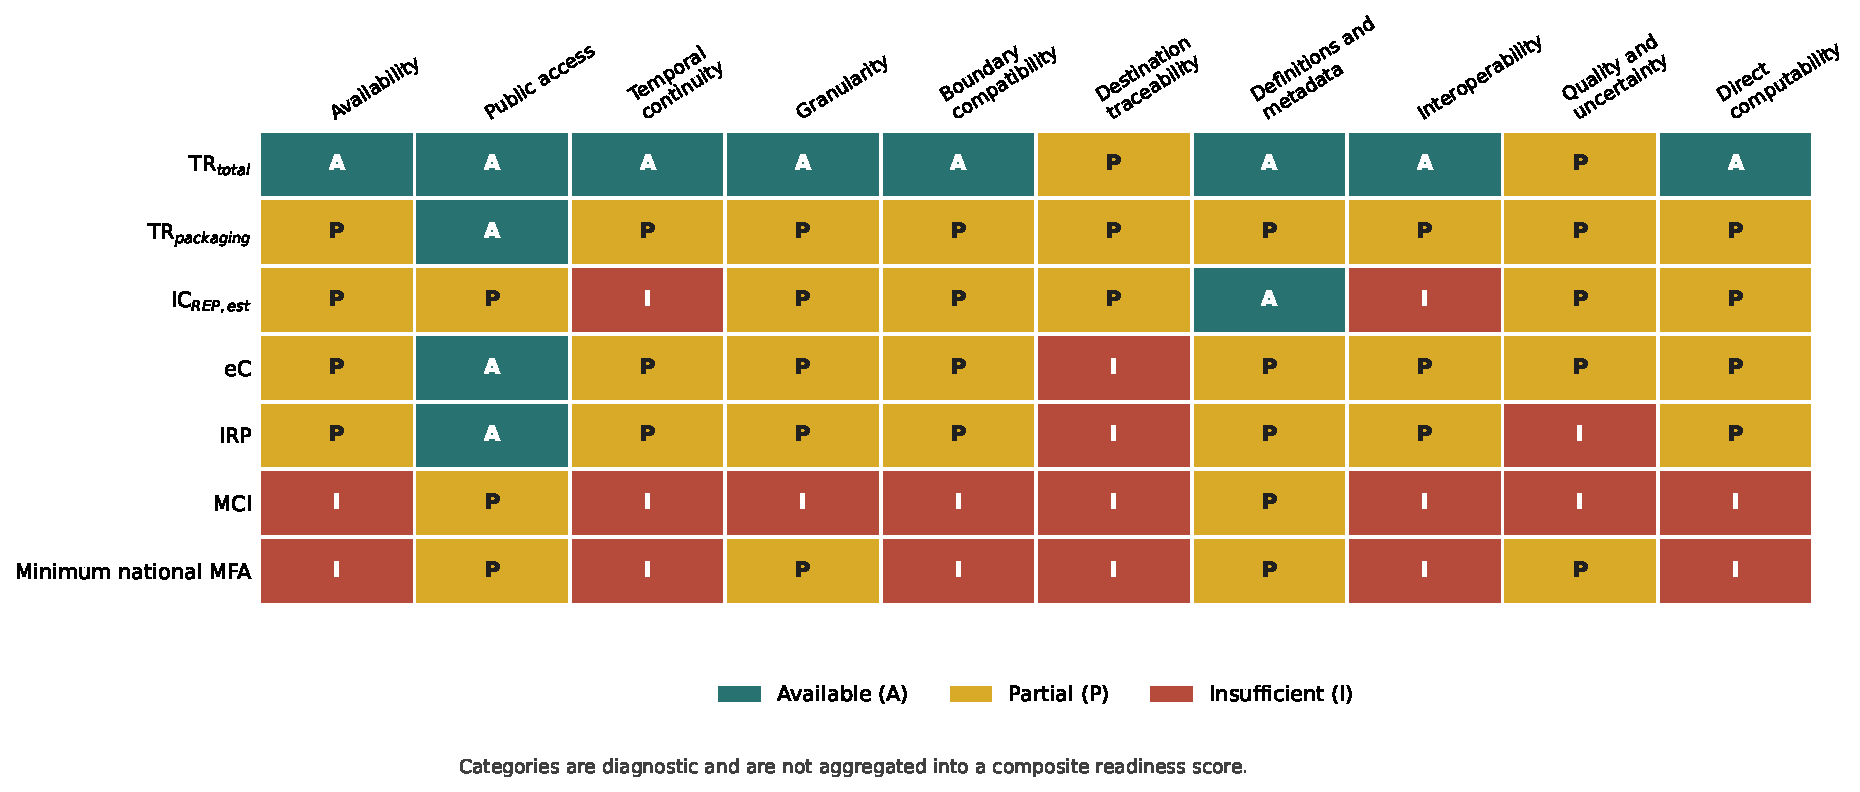
\includegraphics[width=1.0\textwidth]{../figuras/matriz_disponibilidad.pdf}
    \caption{Readiness of publicly accessible information by measurement application and assessment dimension. Categories are diagnostic and are not aggregated into a composite score.}
    \label{fig:readiness_matrix}
\end{figure}

\revpar{The audit does not imply that every required datum is absent from Chilean institutions. It establishes that the required variables were not jointly available to an external user through the public sources examined by the cutoff date and at compatible boundaries. RETC/SINADER provides aggregate waste and destination records; the historical RETC EPR dataset provides grouped priority-product declarations; ANIR studies provide partial material-available, material-managed, and material-unmanaged quantities for selected resins; and ReSimple and GIRO publish system-specific annual results. These sources improve individual segments of the chain but cannot yet be integrated into a national packaging mass balance. Full source-level evidence and the ten-dimension profile are provided in Supplementary Tables S5--S9.}

\revpar{Table \ref{tab:indicadores_resultados} should be read across each row. The first column gives the indicator and unit, the second states its operational meaning, and the annual columns show the time series. TR$_{total}$ uses all apparent plastics consumption, whereas TR$_{packaging}$ uses estimated plastic-packaging input; $T_{gr}$ expresses that packaging input per inhabitant. IC$_{\mathrm{REP,est}}$ is shown only from 2023 onward because packaging targets entered operational implementation that year. Blank cells for 2015--2022 mean \textit{not calculated}, not zero.}

\begin{longtable}{|L{1.9cm}|L{2.1cm}|L{0.85cm}|L{0.85cm}|L{0.85cm}|L{0.85cm}|L{0.85cm}|L{0.85cm}|L{0.85cm}|L{0.85cm}|L{0.85cm}|L{0.85cm}|L{0.85cm}|}
\caption{Circular-economy indicator values for plastic packaging in Chile}
\label{tab:indicadores_resultados}\\
\hline
\textbf{Indicator} & \textbf{Definition} & \textbf{2015} & \textbf{2016} & \textbf{2017} & \textbf{2018} & \textbf{2019} & \textbf{2020} & \textbf{2021} & \textbf{2022} & \textbf{2023} & \textbf{2024} & \textbf{2025} \\
\hline
\endfirsthead
\hline
TR$_{total}$ (\%) & Recycling rate, all plastics & 8.5 & 8.5 & 8.5 & 8.5 & 9.1 & 9.6 & 8.7 & 7.8 & 9.1 & 10.3 & 10.3 \\
\hline
TR$_{packaging}$ (\%) & Recycling rate, plastic packaging & 7.0 & 7.0 & 7.0 & 7.0 & 8.0 & 9.0 & 10.0 & 11.0 & 12.0 & 13.0 & 14.0 \\
\hline
$T_{gr}$ (kg/inhab/year) & Estimated packaging-generation scale & 23.3 & 24.4 & 22.7 & 24.7 & 24.0 & 23.6 & 32.9 & 30.9 & 28.2 & 30.1 & 32.4 \\
\hline
$IC_{\mathrm{REP,est}}$ (\%) & Estimated EPR target attainment &  &  &  &  &  &  &  &  & 84.7 & 82.0 & 68.8 \\
\hline
\end{longtable}

\revpar{The national overview shows different trajectories across dimensions. Packaging recycling rises from 7.0\% in 2015--2018 to 13.0\% in the 2024 reference year, whereas total-plastics recycling fluctuates and reaches 10.3\% in 2024. The estimated per-capita packaging-generation scale also rises to 30.1 kg/inhabitant/year in 2024. IC$_{\mathrm{REP,est}}$ remains below 100\% in every calculated year. These outputs are therefore interpreted separately rather than collapsed into a single score.}

\subsection{Operational Performance Indicators}

\changepar{TR$_{total}$ increased from 8.5\% in 2018 to 10.3\% in 2024. TR$_{packaging}$ increased from 7.0\% to 13.0\% over the same interval. The first percentage is calculated from total recycled plastics divided by total apparent plastics consumption; the second is calculated from recycled plastic packaging divided by estimated packaging input. Stating both denominators prevents the two rates from being read as alternative estimates of the same quantity. In 2024, estimated packaging input was 594,240 tonnes and the population was 19,764,771, producing $T_{gr}=30.1$ kg/inhabitant/year. The provisional 2025 extension yields TR$_{total}=10.3\%$, TR$_{packaging}=14.0\%$, and $T_{gr}=32.4$ kg/inhabitant/year; these values include estimated inputs and are not treated as equally complete evidence.}

\subsection{Estimated EPR Target Attainment (IC$_{\mathrm{REP,est}}$)}

\changepar{IC$_{\mathrm{REP,est}}$ compares estimated recovered plastic packaging in year $t$ with the target rate applied to estimated packaging input in year $t-1$. It is not calculated for 2015--2022 because the packaging obligations entered operational implementation on 16 September 2023; constructing earlier values would imply a regulatory benchmark that was not yet in force. The indicator is 84.7\% in 2023 and 82.0\% in the 2024 reference year. It is 68.8\% in the provisional 2025 extension, where the denominator reflects a higher target and the numerator includes estimated information. These values quantify progress against the study's aggregate national benchmark. They do not establish official compliance, which requires audited legal data disaggregated by obligated entity, management system, target category, and household or non-household origin.}

\subsection{Managed Material Relative to Virgin-Resin Input (eC)}

\changepar{Table \ref{tab:ec_resina} reports $eC_{j,t}=Q_{rec,j,t}/Q_{vir,j,t}$. In the 2024 reference year, the ratio is 0.2193 for PET, 0.3193 for PP, and 0.1685 for PE. Thus, managed material corresponds to approximately 21.9\%, 31.9\%, and 16.9\% of virgin input in the three resin-specific boundaries. These values describe the relative magnitude of two reported or reconstructed flows; they do not establish that the managed material replaced an equivalent quantity of virgin resin. The provisional 2025 values are 0.2030, 0.2654, and 0.1624, respectively. Because $Q_{rec}$ is carried forward from 2024 in the 2025 calculation and selected $Q_{vir}$ values are reconstructed, the 2025 changes should not be interpreted as independently observed shifts in circularity.}

\revpar{The eC table is dimensionless. Rows identify PET, PP, and PE, while columns support within-resin comparison over time. Cross-resin comparisons should remain cautious because each value depends on the coverage and reconstruction of both a resin-specific managed-material numerator and a resin-specific virgin-input denominator.}

\begin{longtable}{|L{1.2cm}|L{1cm}|L{1cm}|L{1cm}|L{1cm}|L{1cm}|L{1cm}|L{1cm}|L{1cm}|L{1cm}|L{1cm}|L{1cm}|}
\caption{\change{Managed material relative to virgin-resin input (eC) for the included resins}}
\label{tab:ec_resina}\\
\hline
\textbf{Resin} & \textbf{2015} & \textbf{2016} & \textbf{2017} & \textbf{2018} & \textbf{2019} & \textbf{2020} & \textbf{2021} & \textbf{2022} & \textbf{2023} & \textbf{2024} & \textbf{2025} \\
\hline
\endfirsthead
\hline
PET & 0.1295 & 0.1283 & 0.1163 & 0.1386 & 0.1689 & 0.1874 & 0.2049 & 0.2155 & 0.2464 & 0.2193 & 0.2030 \\
\hline
PP & 0.2256 & 0.1584 & 0.1377 & 0.0143 & 0.0148 & 0.3492 & 0.3541 & 0.3679 & 0.3090 & 0.3193 & 0.2654 \\
\hline
PE & 0.1246 & 0.1237 & 0.1273 & 0.1197 & 0.1182 & 0.1216 & 0.1198 & 0.1381 & 0.1571 & 0.1685 & 0.1624 \\
\hline
\end{longtable}

\revpar{The eC series is non-monotonic and differs by resin. Variation reflects changes in both managed tonnage and virgin input, not recycling-technology efficiency alone. The very low PP values in 2018--2019 and the increase from 2020 onward should therefore be interpreted together with the underlying data classifications rather than as evidence of an abrupt technological transition.}

\subsection{Impact Reduction Potential (IRP)}

\changepar{Using the emission factors in Table \ref{tab:factores_emision_CO2} and the resin-level managed-material values in Table \ref{tab:irp_resina}, the 2024 calculation yields a positive theoretical impact-reduction potential. IRP is estimated at 0.049902 Mt CO$_2$eq for PET, 0.031717 Mt CO$_2$eq for PP, and 0.093156 Mt CO$_2$eq for PE, for an aggregate theoretical potential of 0.174775 Mt CO$_2$eq across the included resins. This quantity is conditional on the adopted emission factors and the assumed displacement of virgin production; it is not an observed reduction in national emissions.}

\revpar{Table \ref{tab:irp_resina} presents IRP in Mt CO$_2$eq by resin and year. The first three rows report the PET, PP, and PE contributions calculated from their respective emission-factor differences and managed-material quantities. The final row sums those contributions within the common three-resin boundary; it is not an estimate for every polymer consumed in Chile.}

\begin{longtable}{|L{1.2cm}|L{1cm}|L{1cm}|L{1cm}|L{1cm}|L{1cm}|L{1cm}|L{1cm}|L{1cm}|L{1cm}|L{1cm}|L{1cm}|}
\caption{\change{IRP values for the included resins, expressed in Mt CO$_2$eq}}
\label{tab:irp_resina}\\
\hline
\textbf{Resin} & \textbf{2015} & \textbf{2016} & \textbf{2017} & \textbf{2018} & \textbf{2019} & \textbf{2020} & \textbf{2021} & \textbf{2022} & \textbf{2023} & \textbf{2024} & \textbf{2025} \\
\hline
\endfirsthead
\hline
PET & 0.029874 & 0.029874 & 0.031544 & 0.036977 & 0.042736 & 0.046515 & 0.059304 & 0.053494 & 0.055334 & 0.049902 & 0.049902 \\
\hline
PP & 0.012781 & 0.012781 & 0.013037 & 0.001296 & 0.001231 & 0.027602 & 0.031593 & 0.027216 & 0.029729 & 0.031717 & 0.031717 \\
\hline
PE & 0.065792 & 0.065792 & 0.067108 & 0.063440 & 0.060717 & 0.062565 & 0.073424 & 0.074065 & 0.087474 & 0.093156 & 0.093156 \\
\hline
Total, included resins & 0.108447 & 0.108447 & 0.111689 & 0.101713 & 0.104684 & 0.136683 & 0.164320 & 0.154775 & 0.172536 & 0.174775 & 0.174775 \\
\hline
\end{longtable}

\revpar{PE contributes the largest share of the 2024 theoretical total because its managed tonnage is higher, despite PET having the largest emission-factor difference per tonne. The 2025 IRP is numerically unchanged because the resin-level managed-material values are carried forward from 2024 in the revised dataset. The 2025 values should therefore be read as an extension scenario, not as independently observed emissions reductions.}

\revpar{Table \ref{tab:IRP} tests how the 2024 aggregate responds to emission-factor assumptions. The scenario column defines the perturbation; the next two columns report the weighted virgin and recycled factors; the fourth reports aggregate IRP; and the final column measures percentage change from the weighted PET--PP--PE reference case. The $\pm20\%$ scenarios test parameter uncertainty, while the PET-only scenario tests sensitivity to an alternative resin composition.}

\begin{longtable}{|L{4cm}|L{3cm}|L{3cm}|L{3cm}|L{3cm}|}
\caption{Sensitivity analysis of IRP under emission-factor variation, 2024}
\label{tab:IRP}\\
\hline
\textbf{Scenario} & \textbf{Virgin EF (kg CO$_2$eq/t)} & \textbf{Recycled EF (kg CO$_2$eq/t)} & \textbf{IRP (Mt CO$_2$eq)} & \textbf{Variation from reference} \\
\hline
\endfirsthead
\hline
Reference, weighted PET-PP-PE mix & 2,148.08 & 381.62 & 0.174775 & - \\
\hline
Virgin EF -20\%, recycled EF +20\% & 1,718.47 & 457.95 & 0.124717 & -28.6\% \\
\hline
Virgin EF +20\%, recycled EF -20\% & 2,577.70 & 305.30 & 0.224834 & +28.6\% \\
\hline
PET-only scenario & 2,940.00 & 510.00 & 0.240427 & +37.6\% \\
\hline
\end{longtable}

\revpar{IRP remains positive in every scenario, ranging from 0.124717 Mt CO$_2$eq under the conservative factor combination to 0.240427 Mt CO$_2$eq in the PET-only case. These scenarios are deterministic sensitivity tests, not statistical confidence intervals: they show dependence on selected emission factors and resin composition but do not quantify sampling uncertainty or variation among Chilean recycling facilities.}

\subsection{Sensitivity to Data-Completion and Displacement Assumptions}

\revpar{Table \ref{tab:sensitivity_main} summarizes the additional sensitivity tests. Changing the packaging share from 43\% to 53\% changes the 2024 per-capita packaging scale from 26.9 to 33.2 kg/inhabitant/year around the 30.1 reference value. TR$_{packaging}$ remains 13.0\% and IC$_{\mathrm{REP,est}}$ remains 82.0\% because the common share coefficient cancels algebraically under the implemented equations. The result shows that estimated packaging mass is sensitive to this assumption even when the derived ratios are not.}

\begin{longtable}{|L{4.2cm}|L{3.4cm}|L{3.4cm}|L{3.4cm}|}
\caption{Sensitivity of principal outputs to selected assumptions}
\label{tab:sensitivity_main}\\
\hline
\textbf{Assumption and output} & \textbf{Conservative case} & \textbf{Reference case} & \textbf{Upper case} \\
\hline
\endfirsthead
\hline
Packaging share; $T_{gr}$, 2024 & 43\%; 26.9 kg/inhab/year & 48\%; 30.1 kg/inhab/year & 53\%; 33.2 kg/inhab/year \\
\hline
Packaging share; TR$_{packaging}$, 2024 & 43\%; 13.0\% & 48\%; 13.0\% & 53\%; 13.0\% \\
\hline
Packaging share; IC$_{\mathrm{REP,est}}$, 2024 & 43\%; 82.0\% & 48\%; 82.0\% & 53\%; 82.0\% \\
\hline
Virgin displacement; aggregate IRP, 2024 & 50\%; 0.087388 Mt CO$_2$eq & 75\%; 0.131081 Mt CO$_2$eq & 100\%; 0.174775 Mt CO$_2$eq \\
\hline
2025 managed-material treatment & Exclude resin-level 2025 eC and IRP & Carry 2024 $Q_{rec}$ forward and label provisional & Not applicable \\
\hline
\end{longtable}

\revpar{The alternative 2017- and 2022-share allocations leave PET unchanged because its endpoint share is 15\% in both years. For PP, the resulting eC bounds are 0.0139--0.0163 in 2018--2019 and 0.3127--0.3731 in 2020--2021; the year-specific PE bounds remain within 0.1101--0.1305. The complete annual results are provided in Supplementary Table S11. These ranges do not represent measurement error. They isolate the influence of the interpolation rule while holding managed-material quantities and aggregate annual virgin input fixed. The reference interpolation remains the preferred estimate because it avoids imposing either endpoint composition on the entire interval, but the bounds show that PP is more sensitive to resin allocation than PET or PE. Excluding 2025 does not alter any 2024 finding and prevents carried-forward managed material from being mistaken for a new observation.}

\section{Discussion}
\subsection{Divergence between Recovery Monitoring and Material Circularity}

\changepar{The 2024 indicators provide complementary rather than interchangeable evidence. The plastic-packaging recycling rate of 13.0\% describes recovered mass relative to estimated packaging input. IC$_{\mathrm{REP,est}}=82.0\%$ describes progress toward the aggregate target relationship implemented in this study, but does not certify legal compliance. The eC ratio shows that managed material represents 16.9--31.9\% of virgin input across the three included resins, without establishing equivalent reinsertion or substitution. IRP estimates a theoretical environmental potential under transferred emission factors and assumed displacement conditions. At the same time, imported virgin raw material remains substantial at 669,000 tonnes in 2024. The indicators therefore document recovery activity and potential environmental relevance, but their different boundaries and evidential status prevent them from establishing system-wide circularity.}

\changepar{The decision not to publish a numerical MCI strengthens this interpretation. A simplified calculation based on imported virgin resin, estimated packaging input, zero loss terms, and an assumed utility factor would mix incompatible boundaries and systematically favor a higher score. MCI remains relevant because its data requirements expose a governance and interoperability gap in the sources examined: the available reporting does not connect virgin and recycled inputs, unrecovered outputs, process losses, final destinations, and product utility in an auditable material-flow account. The evidence supports a diagnosis of partial measurement readiness rather than a claim that no relevant information exists anywhere in Chile. It also explains why the present results cannot be compared directly with full MFA-based circularity assessments such as those developed for Portugal (Goncalves et al., 2024; Goncalves et al., 2026).}

\subsection{Transferable Minimum Data Architecture for EPR Monitoring}

\changepar{The readiness result is transferable beyond the Chilean case because it identifies the data relationships required to progress from recovery accounting to material-circularity measurement. At minimum, an EPR information architecture should connect: (i) material placed on the market by year, product category, resin, and obligated producer; (ii) collected mass by household or non-household origin; (iii) sorting output and rejected mass; (iv) recycling input, process yield, and losses; (v) imports and exports of waste and secondary resin; (vi) final destinations, including disposal and verified incorporation into new production; and (vii) chain-of-custody identifiers that prevent double counting across producers, management systems, and recovery operators. Definitions, units, reporting periods, revision status, and uncertainty flags should accompany each record. This structure operationalizes the OECD (2024) call to combine material, waste, product, and trade statistics while remaining applicable to EPR systems with different institutional arrangements.}

\changepar{The architecture also clarifies why recovery rates and circularity indicators cannot substitute for one another. Recovery monitoring can function with placed-on-market and recovered masses, whereas eC requires compatible virgin and managed flows, IRP additionally requires destination and displacement evidence, and MCI or MFA requires losses and complete input--output closure. A staged reporting system can therefore preserve operational indicators while progressively adding the fields needed for more demanding measurement applications. The Available, Partial, and Insufficient profile is not a ranking of institutions; it is a map of which data relationships must be added or connected.}

\subsection{The Household-Collection Gap as a System Bottleneck}

\changepar{ASIPLA (2025b) reports that 88\% of recycled plastic in Chile comes from industrial and commercial sources, whereas 12\% originates from household sources. This composition suggests that household collection may be an important system constraint because broader household recovery requires geographically distributed collection, effective source separation, contamination control, and municipal coordination. It also provides context for why progress in an aggregate target-attainment indicator can coexist with total and packaging recycling rates of 10.3\% and 13.0\%, respectively. The present study does not identify the causal contribution of household collection or estimate the additional tonnage obtainable from a higher household share; such analyses would require explicit observations of collection coverage, capture rates, contamination, and processing capacity.}

\subsection{Public-Policy Implications}

\changepar{Two levels of implication must be distinguished. Directly from the audit results, Chilean public reporting would benefit from publishing harmonized target numerators and denominators, resin- and origin-disaggregated flows, sorting and recycling losses, final destinations, and stable identifiers across reporting systems. These are information requirements supported by the observed computability gaps. The results also support retaining 2024 as the reference year, treating 2025 resin-level outcomes as provisional, and refraining from interpreting managed tonnes as verified substitution.}

\changepar{A second level comprises policy instruments proposed in the literature rather than evaluated in this study. Minimum recycled-content requirements and fee modulation may strengthen demand for secondary material, and expanded household collection may increase accessible feedstock, but their effects and costs were not estimated here. They should therefore be treated as hypotheses for policy design and future evaluation, not as causal recommendations demonstrated by the present indicators. Likewise, the 2024 reference IRP of 0.174775 Mt CO$_2$eq is a theoretical potential under complete displacement; the 50\% and 75\% scenarios reduce it to 0.087388 and 0.131081 Mt CO$_2$eq, respectively. Verification of actual destinations and Chile-specific emission factors is required before translating that potential into an emissions-reduction claim.}

\revpar{Table \ref{tab:sintesis} translates the discussion into a decision-oriented summary. Each row corresponds to one analytical dimension. The second column states the principal 2024 finding, with the 2025 extension shown where relevant; the third identifies the evidence or implementation gap that limits interpretation; and the fourth proposes an information or research action consistent with that gap. The table does not claim that the effects or costs of policy instruments were estimated.}

\begin{longtable}{|L{3cm}|L{4cm}|L{4cm}|L{4cm}|}
\caption{Summary of findings, gaps, and recommended actions by dimension}
\label{tab:sintesis}\\
\hline
\textbf{Dimension} & \textbf{Key finding, reference year 2024} & \textbf{Identified gap} & \textbf{Recommended action} \\
\hline
\endfirsthead
\hline
Performance & Plastic-packaging TR = 13\% in 2024 and 14\% in the 2025 extension; 87\% not recovered in 2024 & The functioning recycling flow is predominantly non-household (88\% of recycling). & Measure household collection coverage, capture, contamination, and processing capacity before evaluating expansion instruments. \\
\hline
Regulation & IC$_{\mathrm{REP,est}}$ = 82.0\% in 2024; the provisional 2025 estimate is 68.8\% & Aggregate estimated inputs do not establish official legal compliance. & Publish auditable target numerators and denominators by category, origin, and management system. \\
\hline
Material & eC ranges from 0.1685 for PE to 0.3193 for PP & Resin-level virgin-input values include reconstructed entries; full MCI variables are unavailable. & Improve resin-level input reporting and record unrecovered output, process losses, and product utility. \\
\hline
Environment & Theoretical IRP = 174,775 t CO$_2$eq across the included resins & The estimate depends on transferred factors and assumed displacement of virgin production. & Develop Chile-specific emission factors and trace actual recycled-material destinations before interpreting realized environmental outcomes. \\
\hline
\end{longtable}

\revpar{The synthesis table shows that the four dimensions lead to complementary information requirements. Operational performance points to household collection capacity; IC$_{\mathrm{REP,est}}$ points to legal-data traceability; eC and the MCI feasibility assessment point to resin-level input, destination, and loss-flow reporting; and IRP points to the need for Chile-specific environmental factors and verified displacement conditions.}

\subsection{Limitations and Future Research}

\changepar{The study has six principal limitations. First, the 48\% packaging share converts apparent plastics consumption into estimated packaging input and generation; the 43--53\% scenarios show that this assumption materially changes estimated packaging mass and $T_{gr}$, even though it cancels from two derived ratios. Second, missing annual observations are completed only through documented rules. The endpoint-allocation sensitivity shows that historical PP eC is particularly responsive to reconstructed resin shares. Third, eC and IRP cover PET, PP, and PE rather than the entire polymer mix. Fourth, IRP uses time-invariant European emission factors and unverified displacement; the displacement scenarios therefore represent potential rather than realized impact. Fifth, a full MCI cannot be calculated because $W$, $W_f$, $W_c$, the complete virgin and recycled feedstock fractions, and $F(X)$ are not available at a compatible boundary. Sixth, the readiness audit evaluates information publicly accessible to an external researcher by the stated cutoff date; it does not establish whether unpublished administrative microdata exist or assess their internal quality. Future work should develop a national plastics MFA, publish resin- and origin-disaggregated EPR flows, quantify sorting and recycling losses, construct Chile-specific life-cycle inventories, and replace provisional 2025 values when complete observations become available.}

\section{Conclusion}

\changepar{This study examined both the performance that can be estimated from publicly accessible sources and the readiness of those sources for measuring plastic-packaging circularity in Chile. For the 2024 reference year, the packaging recycling rate was 13.0\% and IC$_{\mathrm{REP,est}}$ was 82.0\%. Managed material represented 16.9--31.9\% of virgin-resin input across PET, PP, and PE, while aggregate IRP was a theoretical 0.174775 Mt CO$_2$eq under the adopted displacement and emission-factor assumptions. The structured audit classified TR$_{total}$ as Available; TR$_{packaging}$, IC$_{\mathrm{REP,est}}$, eC, and IRP as Partial; and MCI and a minimum national MFA as Insufficient. Deterministic sensitivity analysis showed that the packaging-share assumption changes $T_{gr}$ but cancels algebraically from TR$_{packaging}$ and IC$_{\mathrm{REP,est}}$ when applied consistently to both numerator and denominator; historical PP eC is the result most responsive to alternative resin-share reconstructions; and IRP varies linearly with the assumed displacement fraction. These non-interchangeable results document recovery activity and estimated regulatory progress but do not establish official EPR compliance, observed virgin-resin substitution, realized emissions reductions, or system-wide circularity. The provisional 2025 extension is kept separate because several inputs are estimated or carried forward. The central governance gap is therefore not the complete absence of information, but the inability to connect existing institutional, sectoral, and management-system records at compatible material, temporal, and value-chain boundaries. Closing this gap requires interoperable public reporting of placed-on-market quantities, resin-level inputs, recycled content, process losses, and final destinations.}

\section*{Data Availability Statement}

\changepar{A reproducibility package containing the calculation workbook, source inventory, audit documentation, verification and figure-generation scripts, figures, and LaTeX files has been prepared for public release at \url{https://github.com/catalinaarriagada9/PAPER_CIMAC}. External source documents are identified through their institutional access points rather than redistributed without an explicit reuse basis. Repository completeness, licensing, and the permanent archived version will be verified before submission.}

\newpage

\section{References}

\begin{enumerate}[leftmargin=*]

\item \changepar{Andreasi Bassi, S., Boldrin, A., Faraca, G., and Astrup, T. F. (2020). Extended producer responsibility: How to unlock the environmental and economic potential of plastic packaging waste? \textit{Resources, Conservation and Recycling}, 162, 105030. \url{https://doi.org/10.1016/j.resconrec.2020.105030}}

\item \changepar{Antonopoulos, I., Faraca, G., and Tonini, D. (2021). Recycling of post-consumer plastic packaging waste in the EU: Recovery rates, material flows, and barriers. \textit{Waste Management}, 126, 694-705. \url{https://doi.org/10.1016/j.wasman.2021.04.002}}

\item \changepar{Aranda-Uson, A., Portillo-Tarragona, P., Marin-Vinuesa, L. M., and Scarpellini, S. (2019). Financial resources for the circular economy: A perspective from businesses. \textit{Sustainability}, 11(3), 888. \url{https://doi.org/10.3390/su11030888}}

\item \changepar{ASIPLA. (2025a). Estadisticas de la Industria del Plastico 2024. Asociacion Gremial de Industriales del Plastico. \url{https://asipla.cl/asipla-lanzo-las-estadisticas-de-la-industria-del-plastico-2024/}}

\item \changepar{ASIPLA. (2025b). 4to Estudio de Reciclaje y Valorizacion de Plasticos en Chile. Asociacion Gremial de Industriales del Plastico. \url{https://asipla.cl/referentes-tecnicos-de-la-industria-a-traves-de-la-generacion-de-contenido/}}

\item \changepar{Biblioteca del Congreso Nacional de Chile. (2021). Decreto Supremo No. 12/2020, Ministerio del Medio Ambiente: establece metas de recoleccion y valorizacion y otras obligaciones asociadas de envases y embalajes. \url{https://www.bcn.cl/leychile/Navegar?idNorma=1157019}}

\item \changepar{Corona, B., Shen, L., Reike, D., Rosales Carreon, J., and Worrell, E. (2019). Towards sustainable development through the circular economy: A review and critical assessment on current circularity metrics. \textit{Resources, Conservation and Recycling}, 151, 104498. \url{https://doi.org/10.1016/j.resconrec.2019.104498}}

\item \changepar{Czaplicka-Kotas, A., and Kulczycka, J. (2026). Managing Poland's transition to circular economy: Regulatory implementation and governance challenges in the plastic packaging sector. \textit{Sustainability}, 18(4), 1762. \url{https://doi.org/10.3390/su18041762}}

\item \changepar{Dormer, A., Finn, D. P., Ward, P., and Cullen, J. (2013). Carbon footprint analysis in plastics manufacturing. \textit{Journal of Cleaner Production}, 51, 133-141. \url{https://doi.org/10.1016/j.jclepro.2013.01.014}}

\item \changepar{Ellen MacArthur Foundation. (2015). Circularity indicators: An approach to measuring circularity - methodology. Ellen MacArthur Foundation. \url{https://ellenmacarthurfoundation.org/material-circularity-indicator}}

\item \changepar{Eriksen, M. K., and Astrup, T. F. (2019). Characterisation of source-separated, rigid plastic waste and evaluation of recycling initiatives: Effects of product design and source-separation system. \textit{Waste Management}, 87, 161-172. \url{https://doi.org/10.1016/j.wasman.2019.02.006}}

\item \changepar{Goncalves, M., Freire, F., and Garcia, R. (2024). Material flow analysis and circularity assessment of plastic packaging: An application to Portugal. \textit{Resources, Conservation and Recycling}, 209, 107795. \url{https://doi.org/10.1016/j.resconrec.2024.107795}}

\item \changepar{Goncalves, M., Freire, F., and Garcia, R. (2026). Understanding key factors driving circularity in plastic systems through material flow analysis: Findings from Portugal. \textit{Journal of Cleaner Production}, 551, 147941. \url{https://doi.org/10.1016/j.jclepro.2026.147941}}

\item \changepar{Kristensen, H. S., and Mosgaard, M. A. (2020). A review of micro level indicators for a circular economy: Moving away from the three dimensions of sustainability? \textit{Journal of Cleaner Production}, 243, 118531. \url{https://doi.org/10.1016/j.jclepro.2019.118531}}

\item \changepar{Klotz, M., Haupt, M., and Hellweg, S. (2023). Potentials and limits of mechanical plastic recycling. \textit{Journal of Industrial Ecology}, 27(4), 1043-1059. \url{https://doi.org/10.1111/jiec.13393}}

\item \changepar{Leal Filho, W., Barbir, J., Carpio-Vallejo, E., Dobri, A., and Voronova, V. (2025). Decarbonising the plastic industry: A review of carbon emissions in the lifecycle of plastics production. \textit{Science of the Total Environment}, 999, 180337. \url{https://doi.org/10.1016/j.scitotenv.2025.180337}}

\item \changepar{Lopez-Aguilar, J. F., Sevigne-Itoiz, E., Maspoch, M. L., and Pena, J. (2022). A realistic material flow analysis for end-of-life plastic packaging management in Spain: Data gaps and suggestions for improvements towards effective recyclability. \textit{Sustainable Production and Consumption}, 31, 209-219. \url{https://doi.org/10.1016/j.spc.2022.02.011}}

\item \changepar{Ministerio del Medio Ambiente. (2026). Envases y embalajes: Ley REP, decreto de metas e implementacion. \url{https://economiacircular.mma.gob.cl/envases-y-embalajes/}}

\item \changepar{OECD. (2024). \textit{Monitoring Progress towards a Resource-Efficient and Circular Economy}. OECD Publishing, Paris. \url{https://doi.org/10.1787/3b644b83-en}}

\item \changepar{Olatayo, K. I., Mativenga, P. T., and Marnewick, A. L. (2023). Plastic value chain and performance metric framework for optimal recycling. \textit{Journal of Industrial Ecology}, 27(2), 601-623. \url{https://doi.org/10.1111/jiec.13384}}

\item \changepar{Phuang, Z. X., Mulya, K. S., Hoy, Z. X., and Woon, K. S. (2023). Moving towards plastic waste circularity: Redefining extended producer responsibility with externality consideration via P-graph-life cycle optimization framework. \textit{Resources, Conservation and Recycling}, 198, 107187. \url{https://doi.org/10.1016/j.resconrec.2023.107187}}

\item \changepar{Picuno, C., Van Eygen, E., Brouwer, M. T., Kuchta, K., and Thoden van Velzen, E. U. (2021). Factors shaping the recycling systems for plastic packaging waste: A comparison between Austria, Germany and The Netherlands. \textit{Sustainability}, 13(12), 6772. \url{https://doi.org/10.3390/su13126772}}

\item \changepar{Restrepo, F., Ruge, V., Bolanoz, A., and Ortega-Ramirez, A. T. (2026). Measuring Circular Impact: Using LCA to Validate the Environmental Performance of the Circular Vision Packaging Recovery System in Colombia. \textit{Sustainability}, 18(5), 2537. \url{https://doi.org/10.3390/su18052537}}

\item \changepar{Rigamonti, L., and Mancini, E. (2021). Life cycle assessment and circularity indicators. \textit{The International Journal of Life Cycle Assessment}, 26(10), 1937-1942. \url{https://doi.org/10.1007/s11367-021-01966-2}}

\item \changepar{Sassanelli, C., Rosa, P., Rocca, R., and Terzi, S. (2019). Circular economy performance assessment methods: A systematic literature review. \textit{Journal of Cleaner Production}, 229, 440-453. \url{https://doi.org/10.1016/j.jclepro.2019.05.019}}

\item \changepar{Saidani, M., Yannou, B., Leroy, Y., Cluzel, F., and Kendall, A. (2019). A taxonomy of circular economy indicators. \textit{Journal of Cleaner Production}, 207, 542-559. \url{https://doi.org/10.1016/j.jclepro.2018.10.014}}

\item \changepar{Schulte, A., Kampmann, B., and Galafton, C. (2023). Measuring the circularity and impact reduction potential of post-industrial and post-consumer recycled plastics. \textit{Sustainability}, 15(16), 12242. \url{https://doi.org/10.3390/su151612242}}

\item \changepar{Schwarz, A. E., Ligthart, T. N., Bizarro, D. G., De Wild, P., Vreugdenhil, B., and van Harmelen, T. (2021). Plastic recycling in a circular economy: Determining environmental performance through an LCA matrix model approach. \textit{Waste Management}, 121, 331-342. \url{https://doi.org/10.1016/j.wasman.2020.12.020}}

\item \changepar{Solis, M., and Silveira, S. (2020). Technologies for chemical recycling of household plastics: A technical review and TRL assessment. \textit{Waste Management}, 105, 128-138. \url{https://doi.org/10.1016/j.wasman.2020.01.038}}

\item \changepar{Van der Perre, S., Mynko, O., Van Geem, K. M., and Wyns, T. (2024). Modelling of carbon flows in the value chain of packaging plastics in the context of sustainable carbon management. \textit{Sustainable Production and Consumption}, 49, 12-27. \url{https://doi.org/10.1016/j.spc.2024.06.002}}

\item \changepar{Vadoudi, K., Deckers, P., Demuytere, C., Askanian, H., and Verney, V. (2022). Comparing a material circularity indicator to life cycle assessment: The case of a three-layer plastic packaging. \textit{Sustainable Production and Consumption}, 33, 820-830. \url{https://doi.org/10.1016/j.spc.2022.08.004}}

\end{enumerate}

\end{document}
